\documentclass[11pt]{article}
\usepackage[a4paper,margin=2.3cm]{geometry}
\usepackage{amsmath,amssymb}
\usepackage{booktabs}
\usepackage{enumitem}
\usepackage{xcolor}
\usepackage{tikz}
\usepackage{caption}
\usetikzlibrary{arrows.meta,positioning,fit,backgrounds,calc,shapes.geometric}
\usepackage[hidelinks]{hyperref}
\newcommand{\code}[1]{\texttt{\small #1}}

% ---- shared TikZ styles for the figures ----
\tikzset{
  box/.style   ={draw, rounded corners, align=center, minimum height=8mm, font=\small, fill=blue!4},
  hl/.style    ={draw, rounded corners, align=center, minimum height=8mm, font=\small, fill=orange!12, very thick},
  swap/.style  ={draw, rounded corners, align=center, font=\small, fill=red!5, dashed, very thick, draw=red!55},
  vtx/.style   ={circle, draw, minimum size=5.5mm, inner sep=0pt, font=\scriptsize, fill=blue!8},
  arr/.style   ={-{Stealth[length=2.2mm]}, thick},
  epos/.style  ={-{Stealth[length=2mm]}, thick, draw=green!55!black},
  eneg/.style  ={-{Stealth[length=2mm]}, thick, draw=red!60, dashed},
}
\title{\textbf{SAC, TD3, and the HSiKAN backbone}\\[2pt]
  \large How a signed-hypergraph policy is applied to off-policy continuous control}
\author{Dr.\ Csaba Hajdu \\[2pt] \normalsize prepared for Kato-sensei}
\date{2026-06-22}
\begin{document}\maketitle

\begin{abstract}
\noindent A short technical note for the grasping collaboration. It states the two off-policy actor--critic
algorithms we use --- TD3 (deterministic) and SAC (maximum-entropy, stochastic) --- and then shows precisely
how the \emph{HSiKAN} signed-hypergraph network is dropped in as the shared actor/critic representation that
reads the robot's kinematic hypergraph. The methodological point is the clean ablation: \textbf{fix the
algorithm, swap only the backbone} (HSiKAN vs.\ a parameter-matched MLP), so any difference is attributable to
the structure, not to capacity. For the full DDPG\,$\to$\,TD3\,$\to$\,SAC lineage and the newer architectures
(REDQ/TQC/DroQ/CrossQ/TD7), see the companion survey \code{reports/2026-06-21-offpolicy-rl-survey.pdf}; for the
HyMeKo ``MDP-as-data'' substrate see \code{reports/2026-06-21-rl-on-hymeko-technical-report.pdf}. This note is
the application-focused subset.
\end{abstract}

\section{The off-policy contract}
All methods here learn a deterministic or stochastic policy $\pi$ and an action-value critic $Q(s,a)$ from a
replay buffer of transitions $(s,a,r,s',d)$, off-policy. Two conventions matter for robot tasks:
\begin{itemize}[nosep]
  \item \textbf{Twin critics / clipped double-$Q$.} Two critics $Q_1,Q_2$; the target uses
        $\min_i Q_i$ to curb the systematic over-estimation bootstrapping induces.
  \item \textbf{Time-limit truncation is \emph{not} a terminal.} When an episode ends only because it hit the
        step cap, the Bellman target still bootstraps ($d=0$); treating truncation as $d=1$ would teach the
        critic the world ends at the horizon. (This was a real bug we fixed; both trainers now store
        truncation as non-terminal.)
\end{itemize}

\section{TD3 --- twin-delayed deterministic policy gradient}
A deterministic actor $\mu_\theta(s)$ and twin critics. Target actions are smoothed; the actor and target
networks update less often than the critics. With target nets $\bar\mu,\bar Q_i$ and Polyak rate $\tau$:
\begin{align}
  \tilde a' &= \operatorname{clip}\!\big(\bar\mu(s') + \operatorname{clip}(\epsilon,-c,c),\,-a_{\max},a_{\max}\big),
    \quad \epsilon\sim\mathcal N(0,\sigma^2), \\
  y &= r + \gamma(1-d)\,\min_{i=1,2}\bar Q_i(s',\tilde a'), \\
  \mathcal L_{Q_i} &= \big(Q_i(s,a)-y\big)^2, \qquad
  \nabla_\theta J = \nabla_\theta\, Q_1\!\big(s,\mu_\theta(s)\big)\ \text{(every \code{policy\_delay} steps)}.
\end{align}
Three patches over DDPG: (1) clipped double-$Q$, (2) delayed policy/target updates, (3) target-policy
smoothing. TD3 is the reliable deterministic baseline. Exploration is injected as Gaussian \emph{action noise}
at collection time.

\section{SAC --- maximum-entropy, stochastic}
SAC maximises return \emph{plus} policy entropy, $J=\sum_t\mathbb E\big[r_t+\alpha\,\mathcal H(\pi(\cdot|s_t))\big]$.
A squashed-Gaussian actor $a=a_{\max}\tanh(\mu_\phi(s)+\sigma_\phi(s)\odot\varepsilon)$, $\varepsilon\sim\mathcal N(0,I)$,
with the $\tanh$ change-of-variables correction in $\log\pi$; twin soft-$Q$ critics; and the temperature
$\alpha$ auto-tuned to a target entropy $\bar{\mathcal H}=-\dim(a)$:
\begin{align}
  y &= r + \gamma(1-d)\Big(\min_{i}\bar Q_i(s',a') - \alpha\log\pi_\phi(a'|s')\Big), \quad a'\sim\pi_\phi(\cdot|s'),\\
  \mathcal L_\pi &= \mathbb E\big[\alpha\log\pi_\phi(a|s) - \min_i Q_i(s,a)\big], \quad a\sim\pi_\phi(\cdot|s)\ \text{(reparameterised)},\\
  \mathcal L_\alpha &= -\,\mathbb E\big[\log\alpha\,(\log\pi_\phi(a|s)+\bar{\mathcal H})\big].
\end{align}
SAC is the single strongest, most robust continuous-control baseline --- the fair opponent for the structural
policy. \textbf{The entropy term $\alpha\,\mathcal H(\pi)$ is also the research seat:} it is the explicit
insertion point where a HyMeKo-native \emph{structural} entropy of the state hypergraph could later be
substituted or added (a separate experiment; flagged here only so the seat is visible).

\begin{figure}[h]\centering
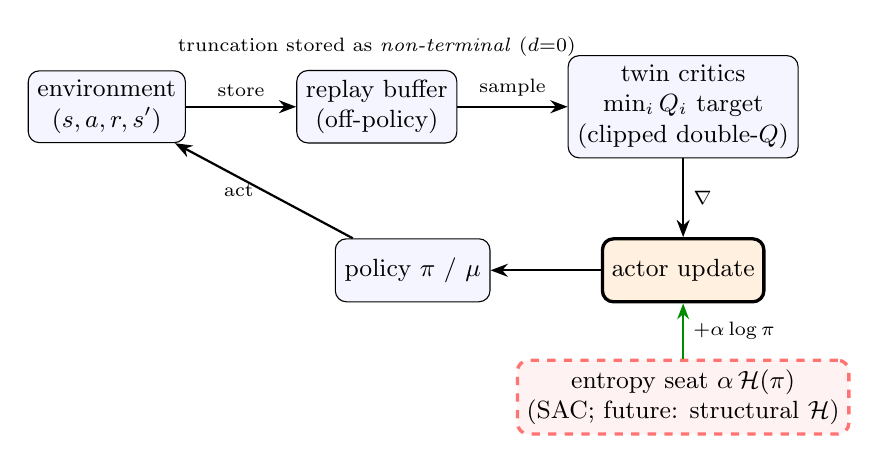
\begin{tikzpicture}[node distance=7mm and 14mm]
  \node[box] (env) {environment\\$(s,a,r,s')$};
  \node[box, right=of env] (buf) {replay buffer\\(off-policy)};
  \node[box, right=of buf] (crit) {twin critics\\$\min_i Q_i$ target\\(clipped double-$Q$)};
  \node[hl, below=10mm of crit] (act) {actor update};
  \node[box, left=of act] (pol) {policy $\pi$ / $\mu$};
  \node[swap, below=7mm of act] (seat) {entropy seat $\alpha\,\mathcal H(\pi)$\\(SAC; future: structural $\mathcal H$)};
  \draw[arr] (env) -- node[above,font=\scriptsize]{store} (buf);
  \draw[arr] (buf) -- node[above,font=\scriptsize]{sample} (crit);
  \draw[arr] (crit) -- node[right,font=\scriptsize]{$\nabla$} (act);
  \draw[arr] (act) -- (pol);
  \draw[arr] (pol) -- node[left,font=\scriptsize]{act} (env);
  \draw[epos] (seat) -- node[right,font=\scriptsize]{$+\alpha\log\pi$} (act);
  \node[font=\scriptsize, above=0.5mm of buf] {truncation stored as \emph{non-terminal} ($d{=}0$)};
\end{tikzpicture}
\caption*{\small\textbf{Fig.~1 — the off-policy loop.} TD3 and SAC share this skeleton; they differ in the
policy (deterministic vs.\ stochastic) and in whether the orange entropy seat is active. The seat is where a
HyMeKo-native structural entropy could later enter.}
\end{figure}

\section{The HSiKAN backbone --- reading the kinematic hypergraph}
The robot is described once in HyMeKo and compiled to a \emph{signed kinematic hypergraph}: vertices are links,
and the signed adjacency $(A^+,A^-)$ encodes the joint connectivity (sign carries the structural relation).
\code{HypergraphState.from\_mjcf} derives $(A^+,A^-)$ from the same source that yields the MuJoCo scene, so the
policy reads the \emph{compiled structure}, not raw joint indices.

\paragraph{Input.} Per-vertex features $x\in\mathbb R^{B\times N\times d}$: each link vertex carries its
dynamic state (e.g.\ $[q,\dot q]$, plus task channels such as the goal vector or the coin direction).

\paragraph{Layer.} One signed graph-conv aggregates self, signed-positive and signed-negative neighbourhoods
(a dense, batched SGCN variant --- kinematic graphs are tiny and the obs is a rollout batch):
\begin{equation}
  h^{(\ell+1)} = \tanh\!\Big(W_{\text{self}}\,h^{(\ell)} \;+\; W_{+}\,(A^{+}h^{(\ell)}) \;+\; W_{-}\,(A^{-}h^{(\ell)})\Big),
\end{equation}
with $A^{\pm}h$ computed as a batched contraction $\sum_m A_{nm}\,h_{b m d}$. After $L$ layers the vertex
embeddings are mean-pooled to a graph embedding $z\in\mathbb R^{B\times \text{hidden}}$.

\begin{figure}[h]\centering
\resizebox{\textwidth}{!}{%
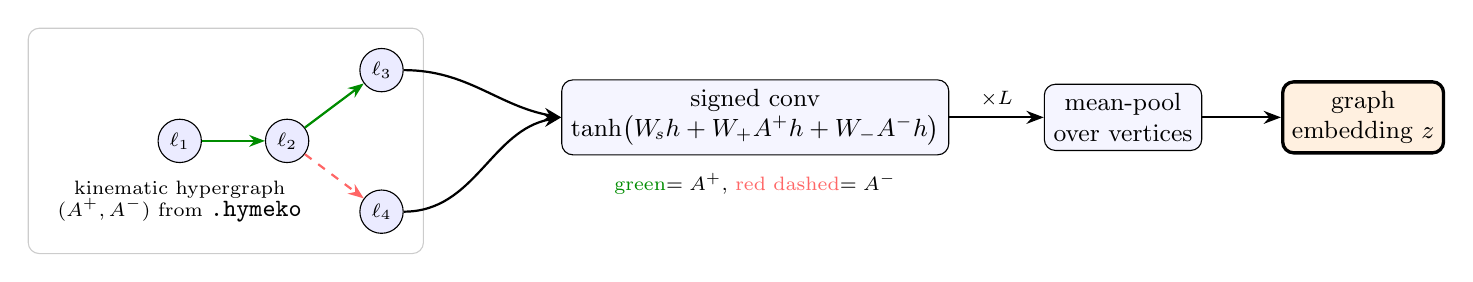
\begin{tikzpicture}[node distance=10mm]
  % kinematic hypergraph (links as vertices; signed edges)
  \node[vtx] (v1) {$\ell_1$};
  \node[vtx, right=8mm of v1] (v2) {$\ell_2$};
  \node[vtx, above right=5mm and 8mm of v2] (v3) {$\ell_3$};
  \node[vtx, below right=5mm and 8mm of v2] (v4) {$\ell_4$};
  \draw[epos] (v1) -- (v2);
  \draw[epos] (v2) -- (v3);
  \draw[eneg] (v2) -- (v4);
  \node[font=\scriptsize, below=1mm of v1, align=center] (cap1) {kinematic hypergraph\\$(A^+,A^-)$ from \code{.hymeko}};
  % the layer
  \node[box, right=20mm of v3, yshift=-6mm] (conv)
    {signed conv\\$\tanh\!\big(W_{\!s}h + W_{+}A^{+}h + W_{-}A^{-}h\big)$};
  \node[box, right=12mm of conv] (pool) {mean-pool\\over vertices};
  \node[hl, right=10mm of pool] (z) {graph\\embedding $z$};
  \draw[arr] (v3.east) to[out=0,in=170] (conv.west);
  \draw[arr] (v4.east) to[out=0,in=190] (conv.west);
  \draw[arr] (conv) -- node[above,font=\scriptsize]{$\times L$} (pool);
  \draw[arr] (pool) -- (z);
  \begin{scope}[on background layer]
    \node[draw=gray!40, rounded corners, fit=(v1)(v2)(v3)(v4)(cap1), inner sep=2.5mm] {};
  \end{scope}
  \node[font=\scriptsize, below=1mm of conv] {\textcolor{green!55!black}{green}$=A^+$, \textcolor{red!60}{red dashed}$=A^-$};
\end{tikzpicture}}
\caption*{\small\textbf{Fig.~2 — HSiKAN signed message passing.} Per-vertex dynamic state is aggregated over the
signed kinematic adjacency (self / positive / negative), $L$ times, then pooled to a fixed-width embedding $z$
that feeds the actor and critic heads.}
\end{figure}

\paragraph{Two variants.}
\begin{itemize}[nosep]
  \item \code{hsikan} --- $A^{\pm}$ are \emph{fixed buffers} (the kinematic structure is given).
  \item \code{signedkan} --- $A^{\pm}$ are \emph{trainable parameters} initialised from the kinematic
        adjacency, so the learned weights \emph{are} the weighted star edges of the hypergraph (the fully
        native ``weights-as-hypergraph'' form).
\end{itemize}

\section{How it plugs into SAC and TD3}
The actor and critic are one shared backbone with two heads (\code{ActorCritic}). The backbone is the swap
point: \code{build\_sac(kind,\dots)} / \code{build\_offpolicy(kind,\dots)} take \code{kind}
$\in\{$\code{hsikan}, \code{signedkan}, \code{mlp}$\}$. The HSiKAN actor outputs $z$ to the SAC squashed-Gaussian
head ($\mu,\log\sigma$) or the TD3 deterministic head ($a_{\max}\tanh$); the critic concatenates $z$ with the
action. \textbf{Nothing in the SAC/TD3 update changes} --- only the representation that reads the state.

\begin{figure}[h]\centering
\resizebox{\textwidth}{!}{%
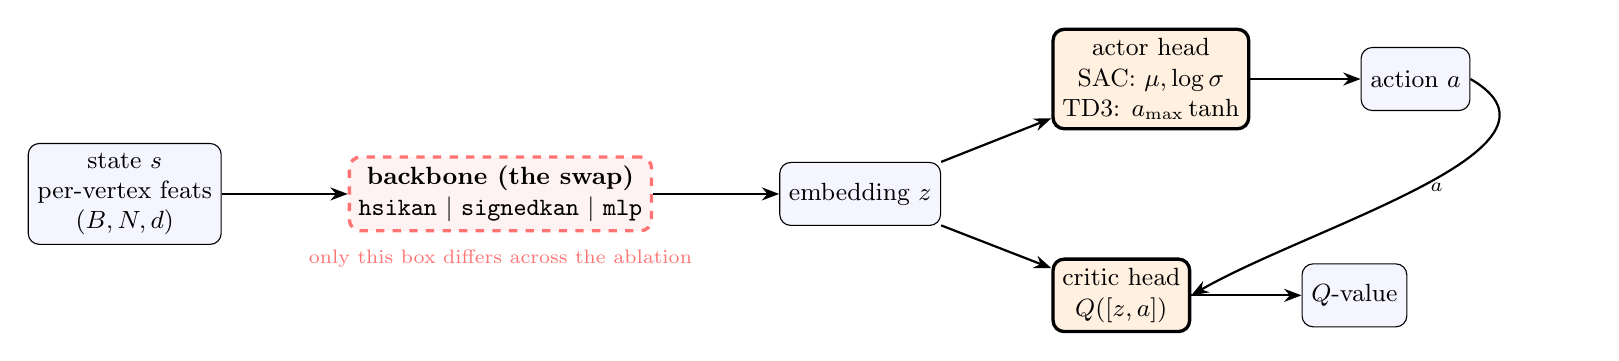
\begin{tikzpicture}[node distance=8mm and 16mm]
  \node[box] (s) {state $s$\\per-vertex feats\\$(B,N,d)$};
  \node[swap, right=of s] (bb) {\textbf{backbone (the swap)}\\\code{hsikan} $\mid$ \code{signedkan} $\mid$ \code{mlp}};
  \node[box, right=of bb] (z) {embedding $z$};
  \node[hl, above right=4mm and 14mm of z] (actor) {actor head\\SAC: $\mu,\log\sigma$\\TD3: $a_{\max}\tanh$};
  \node[hl, below right=4mm and 14mm of z] (critic) {critic head\\$Q([z,a])$};
  \node[box, right=14mm of actor] (a) {action $a$};
  \node[box, right=14mm of critic] (q) {$Q$-value};
  \draw[arr] (s) -- (bb);
  \draw[arr] (bb) -- (z);
  \draw[arr] (z) -- (actor);
  \draw[arr] (z) -- (critic);
  \draw[arr] (actor) -- (a);
  \draw[arr] (critic) -- (q);
  \draw[arr] (a.east) to[out=-30,in=30] node[right,font=\scriptsize]{$a$} (critic.east);
  \node[font=\scriptsize, below=1mm of bb, text=red!55] {only this box differs across the ablation};
\end{tikzpicture}}
\caption*{\small\textbf{Fig.~3 — fix the algorithm, swap the backbone.} The actor and critic share one backbone;
HSiKAN (structure-reading) vs.\ a params-matched MLP (flat) is a single dashed-box swap, so any performance
difference is attributable to the representation, not the algorithm or capacity.}
\end{figure}

\begin{center}\small
\begin{tabular}{lll}
\toprule
role & HSiKAN form & MLP control \\
\midrule
state read & signed message passing over $(A^+,A^-)$ & flattened $(N{\times}d)$ vector \\
actor head & SAC squashed-Gaussian / TD3 $\tanh$ & identical \\
critic & $Q(\,[z,a]\,)$ on the same backbone family & identical \\
\bottomrule
\end{tabular}
\end{center}

\section{The ablation methodology (what the current run measures)}
The question cart-pole could not answer (2 vertices: structure is not load-bearing) is being tested fairly:
\begin{itemize}[nosep]
  \item \textbf{Fix the algorithm, swap the backbone.} HSiKAN vs.\ MLP under one shared SAC.
  \item \textbf{Parameter-matched control.} The MLP width is auto-tuned so its parameter count matches HSiKAN's
        (within $<1.5\%$) per task --- a difference must come from \emph{structure}, not capacity.
  \item \textbf{Real topology, four tasks.} Inverted pendulum (2-vtx, the negative control), Galambos planar
        coin-grasp (6-vtx, Galambos-sensei's scenario), 6-DOF arm reaching (6-vtx), quadruped goal-reaching
        (14-vtx, branching) --- structure grows across the ladder.
  \item \textbf{Honest metric.} \emph{Curve-max} (best mean-return over the eval schedule), reported as
        median\,$\pm$\,IQR\,/\,worst over 5 seeds. A verdict is credited only when the HSiKAN--MLP median gap
        \emph{exceeds the cross-seed IQR}; a gap inside the IQR is a tie, never a single-seed claim.
\end{itemize}
\begin{figure}[h]\centering
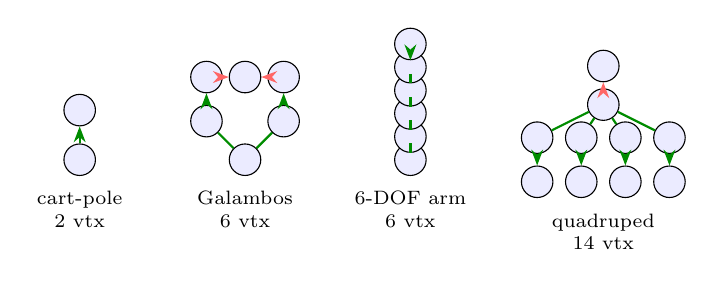
\begin{tikzpicture}[vtx/.append style={minimum size=4mm, font=\tiny}, x=7mm, y=7mm]
  % --- cartpole: 2 vertices ---
  \begin{scope}[shift={(0,0)}]
    \node[vtx] (c1) at (0,0) {}; \node[vtx] (c2) at (0,0.9) {};
    \draw[epos] (c1)--(c2);
    \node[font=\scriptsize, align=center] at (0,-0.9) {cart-pole\\2 vtx};
  \end{scope}
  % --- galambos: 6 vertices (two arms + coin) ---
  \begin{scope}[shift={(3,0)}]
    \node[vtx] (b) at (0,0) {};
    \node[vtx] (l1) at (-0.7,0.7) {}; \node[vtx] (l2) at (-0.7,1.5) {};
    \node[vtx] (r1) at (0.7,0.7) {};  \node[vtx] (r2) at (0.7,1.5) {};
    \node[vtx] (co) at (0,1.5) {};
    \draw[epos] (b)--(l1)--(l2); \draw[epos] (b)--(r1)--(r2);
    \draw[eneg] (l2)--(co); \draw[eneg] (r2)--(co);
    \node[font=\scriptsize, align=center] at (0,-0.9) {Galambos\\6 vtx};
  \end{scope}
  % --- arm6dof: 6-vertex chain ---
  \begin{scope}[shift={(6,0)}]
    \foreach \i in {0,...,5} {\node[vtx] (a\i) at (0,\i*0.42) {};}
    \draw[epos] (a0)--(a1)--(a2)--(a3)--(a4)--(a5);
    \node[font=\scriptsize, align=center] at (0,-0.9) {6-DOF arm\\6 vtx};
  \end{scope}
  % --- quadruped: 14 vertices (torso + 4 two-link legs + base) ---
  \begin{scope}[shift={(9.5,0.4)}]
    \node[vtx] (t) at (0,0.6) {};
    \foreach \dx/\s in {-1.2/lf,-0.4/lb,0.4/rb,1.2/rf} {
      \node[vtx] (\s1) at (\dx,0) {}; \node[vtx] (\s2) at (\dx,-0.8) {};
      \draw[epos] (t)--(\s1)--(\s2);
    }
    \node[vtx] (bj) at (0,1.3) {}; \draw[eneg] (t)--(bj);
    \node[font=\scriptsize, align=center] at (0,-1.7) {quadruped\\14 vtx};
  \end{scope}
\end{tikzpicture}
\caption*{\small\textbf{Fig.~4 — the topology ladder.} Structure grows left to right; the hypothesis is that any
HSiKAN advantage over a flat MLP should also grow with it. Cart-pole is the negative control (structure not
load-bearing).}
\end{figure}

Prior single-seed evidence (cart-pole, and a first Galambos run) showed \emph{parity} with matched capacity,
with a whiff of HSiKAN parameter-efficiency only as topology got rich (quadruped). The multi-seed off-policy run
now in flight is what turns that into a firm statement; results tables (\code{booktabs}, drop-in) are generated
automatically from the run journal.

\section{Why this matters for the grasping collaboration}
The deliverable is a \emph{structurally accountable} control head: the same HyMeKo hypergraph that describes the
robot is what the policy reads, the policy network itself round-trips back to HyMeKo, and the comparison against
a matched MLP is built in --- so a claim that ``the structure helps'' is always testable, never asserted. If the
edge widens on the richer-topology tasks (the hand / contact graphs in grasping are far richer than these
testbeds), that is the first real signal that reading the kinematic structure --- rather than a flat state ---
earns its place.

\end{document}
